\documentclass[a4paper,12pt]{CSUResearchProposal}
\usepackage[top=2.4cm, bottom=3cm, left=2.5cm, right=2.5cm]{geometry}
\usepackage{indentfirst}
\usepackage{extpfeil}
%\usepackage{times}  % Times fonts
\usepackage{titlesec}
\usepackage{hyperref}
\usepackage{graphicx}
\usepackage{subfigure}
%\usepackage[ruled,vlined,norelsize]{algorithm2e}
\usepackage{esint}
\usepackage{paralist}
\usepackage{enumerate}
\usepackage{amssymb,amsmath}
\usepackage{amsbsy}
\usepackage{amsthm}
\usepackage{type1cm}
\usepackage{type1ec}
\usepackage{background}
\usepackage{graphicx}

% 全局设置背景图片
\backgroundsetup{
    scale=1, % 缩放系数
    angle=0, % 旋转角度
    opacity=0.6, % 透明度
    contents={%
        
\includegraphics[width=\paperwidth,height=\paperheight,keepaspectratio]{./figures/csu_bg.jpg}
    }
}


%\usepackage[a4,frame,center]{crop}
%\usepackage{noinfo}
% \usepackage{stmaryrd}
%\usepackage[square,sort,comma,numbers]{natbib}
\usepackage{natbib}
%\usepackage{javen}
\usepackage{bbm}
\bibliographystyle{model5-names}

\newcommand{\NP}{\mathcal{NP}}

% \xeCJKsetup{CJKglue=\hspace{0pt plus .08 \baselineskip }}  
%\titleformat{\section}{\Large\bfseries}{\thesection.}{1em}{}


\linespread{1.56}

\usepackage{float}
\usepackage{algorithm}
\usepackage{algorithmicx}
\usepackage{algcompatible}
\floatname{algorithm}{\zihao{-5}算法}
\renewcommand{\algorithmicrequire}{\textbf{输入:}}
\renewcommand{\algorithmicensure}{\textbf{输出:}}
\begin{document}
\author{XXX}
\StudentID{12345678}
\ThesisTitle{开题报告模板}
\SubjectFrom{学校自选题目}
\School{计算机学院}
\Major{人工智能}
\Degree{工学博士学位}
\Supervisor{xxx~教授}
\Date{2024年12月12日}

% 注意这里需要手写,所以需要去掉
% \ReviewerOne{A}{教授}{XXX学院}
\ReviewerOne{ }{ }{ }
\ReviewerTwo{ }{}{ }
\ReviewerThree{ }{ }{ }
\ReviewerFour{ }{ }{ }
\ReviewerFive{ }{ }{ }
\ReviewerSix{ }{ }{ }

\Secretary{ }{ }{ }
\maketitle



\section{选题意义和研究价值}
\label{sec:background}
参考文献示例\citep{han2024cancer}.

公式示例
\begin{equation}\label{equ:potential}
V = G\rho \iiint\limits_\Omega  {\frac{1}{{\sqrt {\Delta x_1^2 + \Delta x_2^2 + \Delta x_3^2} }}d\Omega }
\end{equation}

图片示例
\begin{figure}[H]
	\centering
	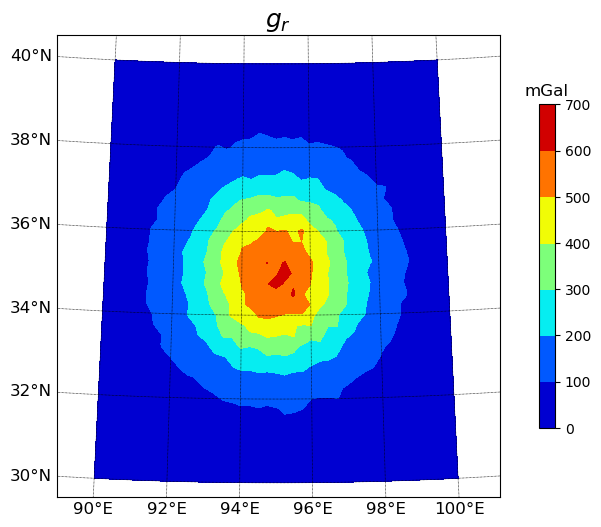
\includegraphics[width=0.6\linewidth]{figures/gr}
	\caption{图片示例}
	\label{fig:gr}
\end{figure}


\newpage
  
\section{国内外研究现状和发展动态}
\label{sec:current_state}

\newpage


\section{主要研究思路、研究内容和在学术方面的创新点}
\label{sec:contents_research}

\newpage

\section{拟采取的研究方法和技术路线}
\label{sec:method}


\newpage

\section{进度安排和预期成果}

\newpage

\section{已有基础{\kaishu (与本项目有关的工作积累和已取得的成绩、已具备的条件、尚缺少的条件及解决途径)}}


\newpage

\section{主要参考文献}
\vspace*{-3ex}
\bibliographystyle{unsrt}
\bibliography{ref}
%\bibliographystyle{IEEEtranN}   % (uses file "plain.bst")
%\bibliography{ref}      % expects file "myrefs.bib"

\end{document}

%%% Local Variables: 
%%% coding: utf-8
%%% mode: latex
%%% TeX-engine: xetex
%%% End: 